\documentclass[11pt]{beamer}
\usepackage[english]{babel}
\usepackage{graphicx, subfig} 
\usepackage{booktabs, fontspec, xcolor,hyperref, pifont}  
\date{\today}
\newcommand{\done}{\rlap{$\square$}{\raisebox{2pt}{\large\hspace{1pt}\ding{51}}}%
    \hspace{-2.5pt}}
\newcommand{\fail}{\rlap{$\square$}{\large\hspace{1pt}\ding{55}}}
\newcommand{\pend}{\rlap{$\square$}{\raisebox{2pt}{\large\hspace{1pt}}}%
    \hspace{6.5 pt}}
\mode<presentation> {
\usecolortheme{beaver}
}
\setromanfont[
BoldFont=QuattrocentoSans-Bold.ttf,
ItalicFont=QuattrocentoSans-BoldItalic.ttf,
BoldItalicFont=QuattrocentoSans-Italic.ttf
]{QuattrocentoSans-Regular.ttf}
\setsansfont[
BoldFont=QuattrocentoSans-Bold.ttf,
ItalicFont=QuattrocentoSans-BoldItalic.ttf,
BoldItalicFont=QuattrocentoSans-Italic.ttf
]{QuattrocentoSans-Regular.ttf}

\author[Dacastillo]{Daniel Castillo Castro} 
\begin{document}
\everymath{\color{blue}}
\everydisplay{\color{blue}}
\title[aC-WR1]{aC Weekly Report 1} 
\begin{frame}
\titlepage 
\end{frame}
\begin{frame}{Bulk Modulus in Lammps}
Part of materials elastic properties (very underrated in academic teaching).
\begin{equation} \label{Bulk} K=-V\frac{dP}{dV}\end{equation}
$P$=Pressure, $V$=Volume \\
It can be obtained by 2 ways:
\begin{itemize}
    \item Using script \textcolor{green}{in.elastic} 
    \item Calculating slope after expand and compress the sample.
\end{itemize}
\end{frame}
\begin{frame}{Script method}
\begin{itemize}
    \item Script \textcolor{green}{in.elastic} is linked with the scripts:
    \begin{itemize}
        \item \textcolor{green}{init.mod}: Read the initial sample (aC made by \textcolor{green}{in.marks}
        \item \textcolor{green}{potential.mod}: Defines potential to use (EDIP in next results)
        \item \textcolor{green}{displace.mod}: Define compression and expansion required for calculus.
    \end{itemize}
    \item Pro: Gives data results faster and more automatically.
    \item Cons: The algorithm is more complex.
\end{itemize}
\end{frame}
\begin{frame}{Slope Method}
\begin{itemize}
    \item Start expanding and compressing the sample using \textcolor{green}{Lammps}. 
    \item Taking the slope of program evolution, $\frac{dp}{dV}$ is given. Multiplying by initial module it can be obtained $K$
    \item Pro: Easier implementation.
    \item Cons: More probability of human mistakes.
\end{itemize}
\end{frame}
\begin{frame}{Compression and Expansion Process}
\begin{figure}
 \centering
    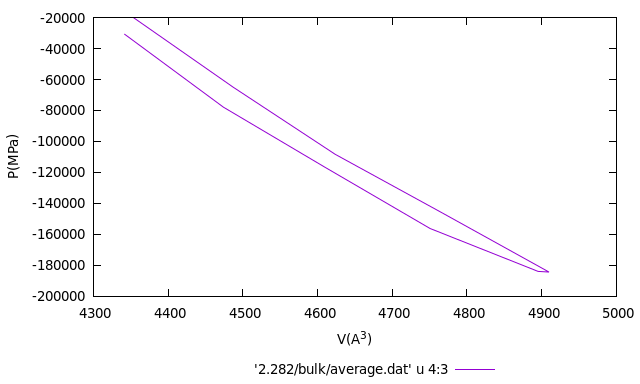
\includegraphics[width=0.8\textwidth]{plot-bulk.png}
 \caption{Process of Compression and Expansion of a sample of aC of initial density $\rho=2.808\frac{g}{cm^3}$, passing between volumes of $4900 A^3$ to $4300 A^3$. Used to find $K$ via slope method.}
\end{figure}
\end{frame}
\begin{frame}{First Running: Results}
\begin{figure}
 \centering
    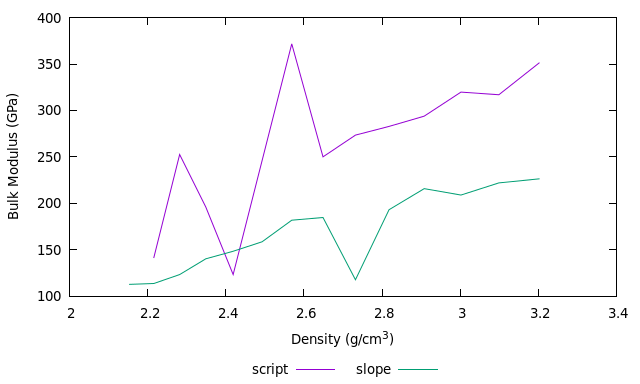
\includegraphics[width=0.9\textwidth]{plot-yeah.png}
 \caption{Bulk Modulus calculations using script method (pink line) and slope method (blue line). Great difference between the two results}
\end{figure}
\end{frame}
\title[aC-WR2]{aC Weekly Report 2} 
\begin{frame}
\titlepage 
\end{frame}
\begin{frame}{First Running: Analysis}
\begin{itemize}
    \item Why they are so different? $\textcolor{red}{\Rightarrow}$ 2 reasons:
          \begin{itemize}
          \item The both methods needs to be modified (The evolución must be linear and not oscillating).
          \item The metods works for differents temperatures (the script one at $T = 0K$, slope one at $T \sim 300K$).
          \end{itemize}
    \item Possible Solutions
    \begin{itemize}
    \item Correction to the both metods
    \item The both methods must to work at $T \sim 0K $
    \end{itemize}
\end{itemize}
\end{frame}
\begin{frame}{Slope Method Corrections}
\begin{itemize}
    \item Improve data analysis considering 
    \begin{equation}\label{slope}K=\frac{m*V}{0.0001\frac{bar}{GPa}}\end{equation}
    ($m$: curve slope in $\frac{atm}{A^3}$, $V$: volume in $A^3$)
    \item Change Temperature from $300K$ to $0K$ looking for results more similar to the script ones.
    \item Low compression and expansion rate from $5\%$ to $1\%$, looking for a curve more linear.
\end{itemize}
\end{frame}
\begin{frame}{Script Method Corrections}
\begin{itemize}
    \item Running it again (for consideration of random effects)
    \item Read input file and check its correctness
    \item It was observed \textcolor{red}{3 densities with incorrect data}. It was proceed to correct it.
\end{itemize}
\end{frame}
\begin{frame}{Corrected Compression and Expansion Process}
\begin{figure}
 \centering
    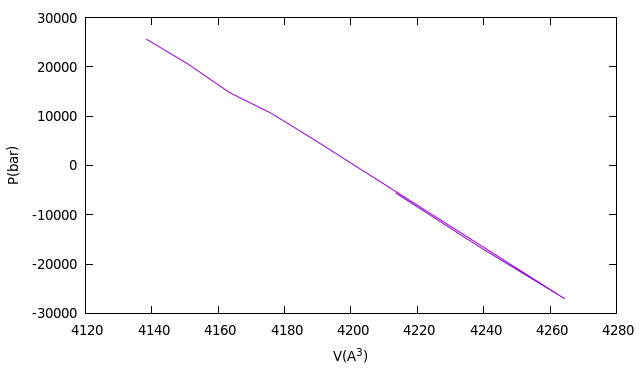
\includegraphics[width=0.8\textwidth]{plot-bulk2.png}
 \caption{New Compression and Expansion process por the sample with $\rho=2.808\frac{g}{cm^3}$, going between $4120 A^3$ to $4270 A^3$. Used for slope method for $K$ calculation.}
\end{figure}
\end{frame}
\begin{frame}{Second Running: Results}
\begin{figure}
 \centering
    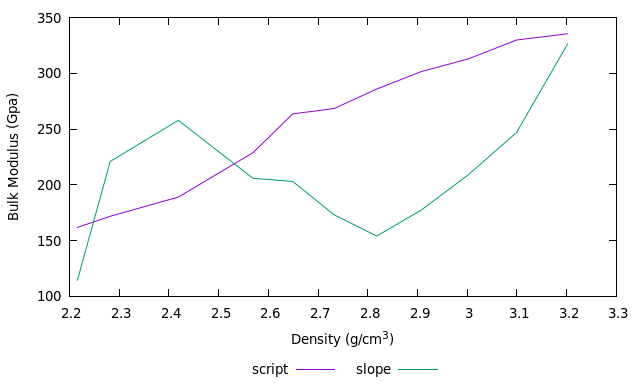
\includegraphics[width=0.9\textwidth]{plot-yeah2.png}
 \caption{Bulk Modulus calculations using script method (pink line) and slope method (blue line). Results generated with 12 cores.}
\end{figure}
\end{frame}
\begin{frame}{Second Running: Analysis}
\begin{itemize}
    \item Script Method obtains data that suggest a linear evolution (correct according to references)
    \item Slope Method \textcolor{red}{doesn't}. Even worse: Some result seems to be failed.
    \item Can de cores number affect the result? (With few the running could be slow, with too much could be clumpsy).
    \item What results will be obtained if core quantity is reduced? (from 12 to 8)
\end{itemize}
\end{frame}
\title[aC-WR3]{aC Weekly Report 3} 
\begin{frame}
\titlepage 
\end{frame}
\begin{frame}{Third Running, Results}
\begin{figure}
 \centering
    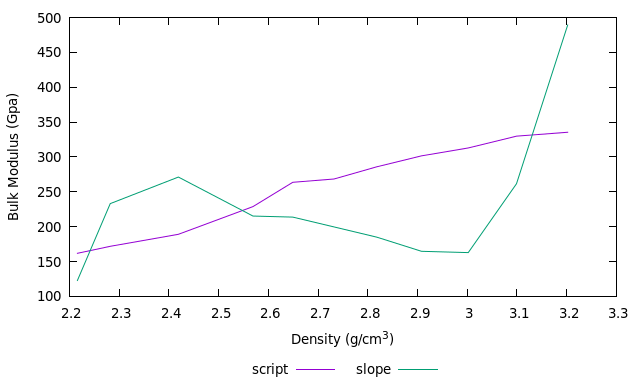
\includegraphics[width=0.9\textwidth]{plot-yeah3.png}
 \caption{Bulk Modulus calculations using script method (pink line) and slope method (blue line). Results generated with 8 cores}
 \end{figure}
\end{frame}
\begin{frame}{Third Running, Analysis}
\begin{itemize}
    \item Data dispersion changes, but is not enough for the expectations.
    \item 1 possible option: lowering cores number even more (from 8 to 4)
    \item If this doesn't works, it will be needed another hypotesis.
    \item Effects of randomness of aC?
\end{itemize}
\end{frame}
\begin{frame}{Correction for the Fourth Running}
\begin{itemize}
    \item Correction to density values in analysis because volume changes after initial relaxation in the both methods:
    \begin{equation}\rho=\frac{m}{V}=\frac{m}{V_0}\frac{V_0}{V}\end{equation}
    ($\rho$: Density, $m$: Mass, $V_0$: Volume used before, $V$: Volume after relaxation)
    \item Give to script method mode time to relaxation process (it wasn't enough for reaching acceptable results).
    \item Use of \textcolor{green}{XMgrace} for fitting in slope method (\textcolor{green}{Gnuplot} fails).
    \item Improvement of data visualizacion of Bulk Modulus in \textcolor{green}{Gnuplot}.
\end{itemize}
\end{frame}
\begin{frame}{Fourth Running: Results}
\begin{figure}
 \centering
    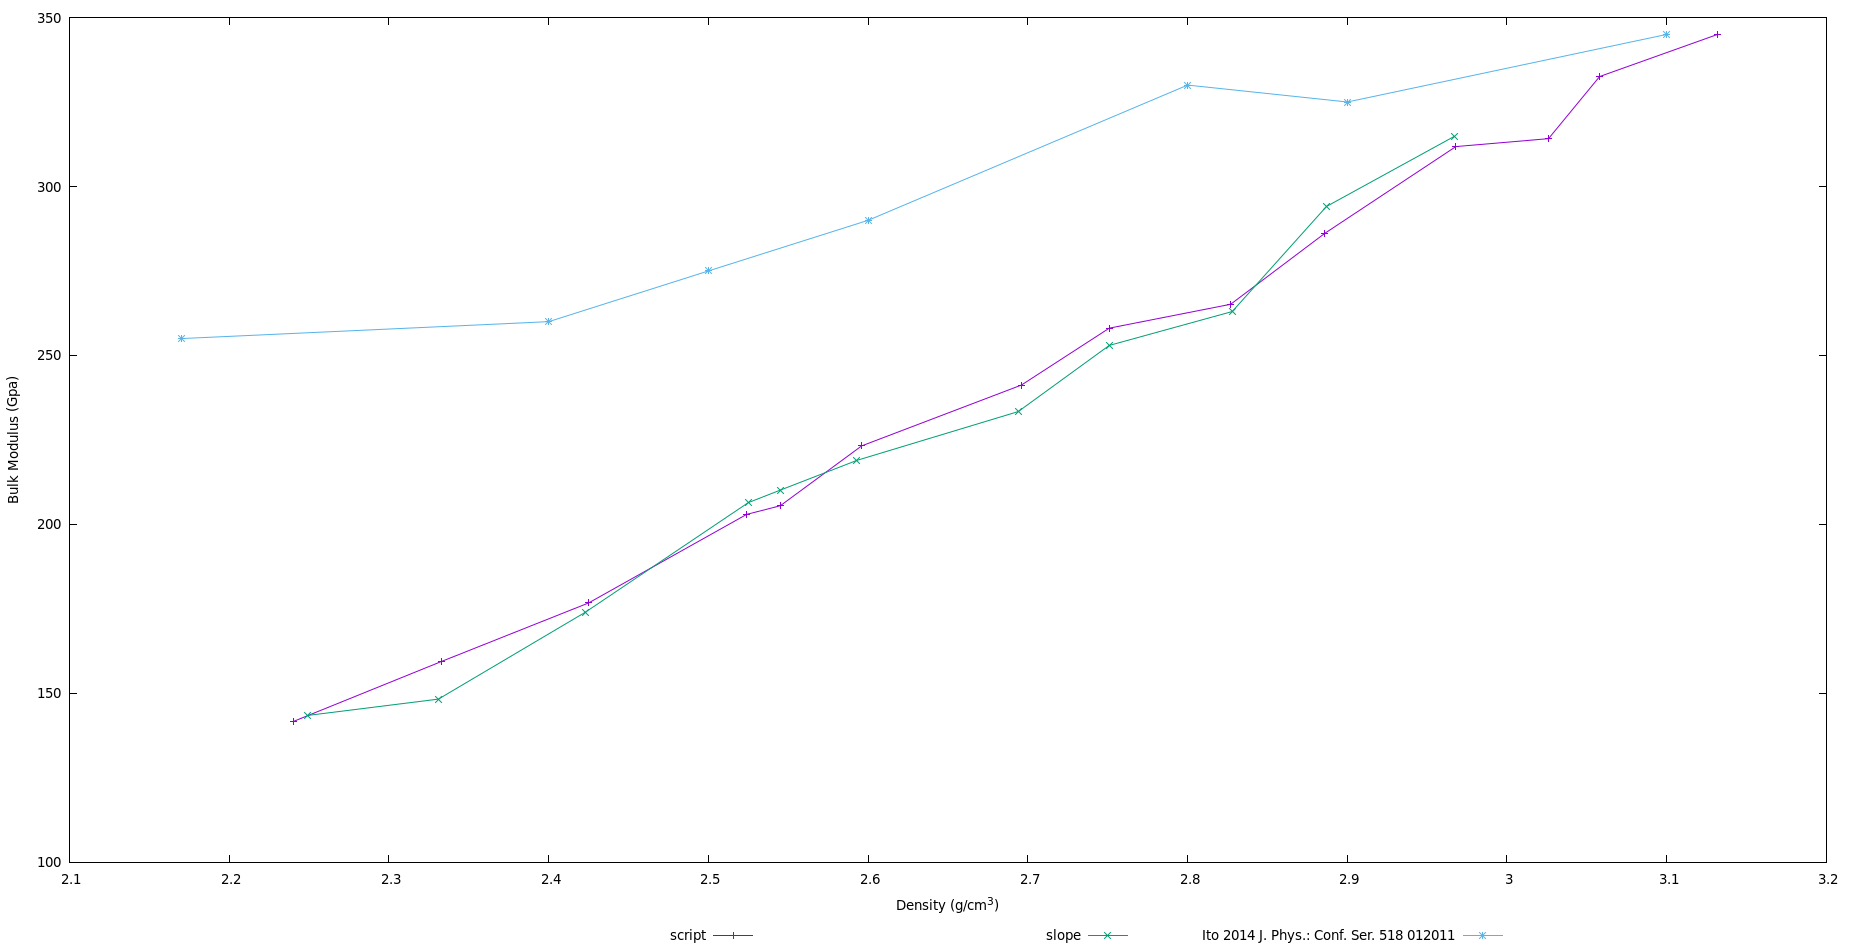
\includegraphics[width=0.9\textwidth]{plot-yeah4.png}
 \caption{Bulk Modulus calculations using script method (pink line) and slope method (blue line). The both methods reach similar results.}
 \end{figure}
\end{frame}
\begin{frame}{Challenges from future research}
\begin{itemize}
    \item The both methods gives similar results, but there are lower than the results of Ito (Possible reason: it is a simulation with room temperature)
    \item There is a \textcolor{green}{in.elastic} script that includes variable temperature. Use it and tune it for the existing samples 
    \item Compare the resuls of this script with Bulk Modulus calculations by slope method at room temperature ($T=300K$)
    \item Look for and use another methods existing in \textcolor{green}{Linux/Ubuntu} for linear regression.
\end{itemize}
\end{frame}
\begin{frame}{Projections of Research}
\begin{itemize}
    \item Make temperature ramps for all the existing ramps for search phase changes. Comparing it with Zazula.
    \item Using \textcolor{green}{Ovito}, checking out the coordination numbers for all the samples made.
    \item Using the elastic scripts, take the standard deviation of Young moduli in the 3 directions.
    \item Make several measurements for avoid random errors.
\end{itemize}
\end{frame}
\title[aC-WR4]{aC Weekly Report 4} 
\begin{frame}
\titlepage 
\end{frame}
\begin{frame}{in.elastic tuning}
\begin{itemize}
    \item The script for $T\neq 0$ has more variables to tune for having an adequate result.
    \item Expected result: a linear increase of Bulk Moduli, a little bit greater than the $T=0$ case.
    \item The example script for the new case is found in folder \textcolor{green}{lammps/tree/master/examples/ELASTIC\_T}.
    \item Taken the example, it was adapted for the case of the aC Lattice obtained before.
\end{itemize}
\end{frame}
\begin{frame}{in.elastic tuning}
\begin{itemize}
    \item Variables tuned for the script:
    \begin{itemize}
        \item \textcolor{green}{up}: Expansion of the material (it must be a very little number).
        \item \textcolor{green}{nrepeat}: Number of samples (it can be any quantity for fitting).
        \item \textcolor{green}{nevery}: Sampling interval (it can be greater).
    \end{itemize}
    \item After one week of changing this variables and running the scripts again (for \textcolor{green}{EDIP} potential) it couldn't be obtained a satisfactory result.
    \item What change can make the script to generate correct results? It has be needed another kind of change?
\end{itemize}
\end{frame}
\begin{frame}{in.elastic tuning}
\begin{itemize}
    \item Another variables that could be tuned:
    \begin{itemize}
        \item \textcolor{green}{timestep}: Time used for every program run (Is enough time to take the result?)
        \item \textcolor{green}{tdamp}: Time constant for thermostat (Can affect the result?)
        \item \textcolor{green}{neighbor}: Can some weird neighbor behaviour set by the script damage the data?
    \end{itemize}
    \item It was advised by Rafael that nonzero temperature script gives more errors to take the result.
    \item Is the results of room temperature fit with Ito's results? 
\end{itemize}
\end{frame}
\begin{frame}{New Slope Methods}
\begin{itemize}
    \item Linear Regression in \textcolor{green}{Gnuplot} fails. But why?
    \item Meanwhile, using \textcolor{green}{XMGrace} the results of Linear Regression seems more adequated.
    \item But \textcolor{green}{XMGrace} has a disadvantage: Is an old programm and can't run without GUI.
    \item Can I find a method via console that gives good results for Linear Regression?
\end{itemize}
\end{frame}
\begin{frame}{New Slope Mehtods}
\begin{itemize}
    \item A possible candidate: Ubuntu commands like \textcolor{green}{gmtgress} or \textcolor{green}{gblred}
    \item Advantage: Looks ligther to run,, simpler to put in \textcolor{green}{bin bash} scripts.
    \item Disadvantage: Can give results with more errors (this is not a science base program). 
    \item Can this kind of methods to be able to run datafiles like \textcolor{green}{Lammps} output files?
\end{itemize}
\end{frame}
\begin{frame}{New Slope Methods}
\begin{itemize}
    \item Another candidate: A \textcolor{green}{Python} script.
    \item Libraries used: \textcolor{green}{Pandas} (data reading), \textcolor{green}{Scikit} (Realisation of Linear Regression Algorithm).
    \item Advantage: Can take datafiles using typical \textcolor{green}{Python} methods
    \item Disadvantage: It could be new errors related with arrange analysis.
\end{itemize}
\end{frame}

\title[NV-aC5]{aC Weekly Report 5} 
\begin{frame}
\titlepage 
\end{frame}
\begin{frame}{Development of To-Do list}
\begin{itemize}
\item bla
\begin{itemize}
\item[\done] blub
\item[\fail] bla
\item[\pend] blo
\end{itemize}
\item blub
\end{itemize}
\end{frame} 

\title[NV-aC6]{aC Weekly Report 6} 
\begin{frame}
\titlepage 
\end{frame}
\begin{frame}{Development of To-Do list}
\begin{itemize}
\item bla
\begin{itemize}
\item[\done] blub
\item[\fail] bla
\item[\pend] blo
\end{itemize}
\item blub
\end{itemize}
\end{frame} 

\title[NV-aC7]{aC Weekly Report 7} 
\begin{frame}
\titlepage 
\end{frame}
\begin{frame}{Development of To-Do list}
\begin{itemize}
\item bla
\begin{itemize}
\item[\done] blub
\item[\fail] bla
\item[\pend] blo
\end{itemize}
\item blub
\end{itemize}
\end{frame} 

\title[NV-aC8]{aC Weekly Report 8} 
\begin{frame}
\titlepage 
\end{frame}
\begin{frame}{Development of To-Do list}
\begin{itemize}
\item bla
\begin{itemize}
\item[\done] blub
\item[\fail] bla
\item[\pend] blo
\end{itemize}
\item blub
\end{itemize}
\end{frame} 
\title[NV-WR1]{NV Centers Weekly Report 1} 
\begin{frame}
\titlepage 
\end{frame}
\begin{frame}{NV Centers State of Art}
\begin{itemize}
    \item NV Center are very required for quibit representation.
    \item It can be possible to simulate and evaluate mechanical and vibrational properties using Classical Molecular Dynamics (\textcolor{green}{LAMMPS}).
    \item Is possible to add quantum effects in a Classical MD simulation, without using \textcolor{green}{DFT}?
\end{itemize}
\end{frame}
\begin{frame}{4 possible NV Centers Hamiltonian}
\begin{itemize}
    \item Static Magnetic Field in $\hat{z}$
    \begin{equation}H=DS_Z^2+\gamma_e B_zS_z\end{equation}
    \item Arbitrary Magnetic Field
    \begin{equation}H=DS_Z^2+\gamma_e \vec{B}\cdot\vec{S}\end{equation}
    \item Static Magnetic Field in $\hat{z}$ and Nuclear Spin
    \begin{equation}H=DS_Z^2+\gamma_e B_zS_z+\gamma_n B_zI_z+S_zA_{zz}I_{z}\end{equation}
    \item Static Magnetic Field in $\hat{z}$, Nuclear Spin and Anisotropy
    \begin{equation}H=DS_Z^2+\gamma_e B_zS_z\gamma_n B_zI_z+S_zA_{zz}I_{z}+\frac{A_{ani}}{2}S_z(I_++I_-)\end{equation}
\end{itemize}
\end{frame}
\begin{frame}{How to read the Hamiltonian?}
\begin{itemize}
    \item The electron spin of the defect in diamond is the qubit implementation.
    \item Electronic and Nuclear Spin can be affected by a Magnetic Field
    \item The dynamics given by the Hamiltonian explain the coherence and correlation of state in time evolution
    \item Trying to reproduce the phonon relaxation rates and energy levels of the system could be interesting.
\end{itemize}
\end{frame}
\begin{frame}{Phonon Relaxation Rates}
\begin{figure}
 \centering
    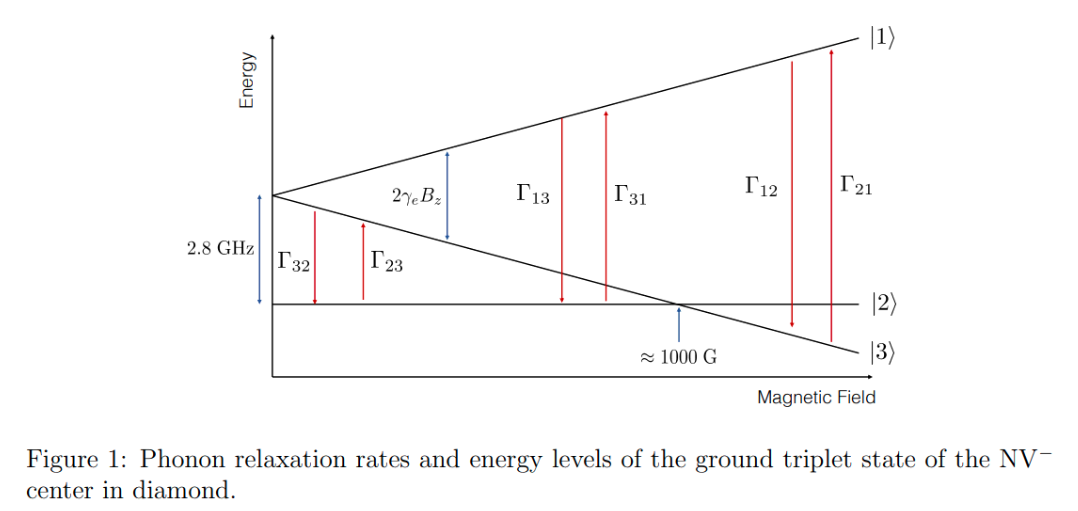
\includegraphics[width=0.8\textwidth]{phononic.png}
    \caption{Representation of the reaction to an Spin Magnetic Field to an NV Center System. Taken from an internal script of Norambuena and Coto (in Dropbox Folder). This indicates that adding a external magnetic field to the MD system would be needed.} 
 \end{figure}
\end{frame}
\begin{frame}{NV Centers MD Realisation.}
\begin{figure}
 \centering
    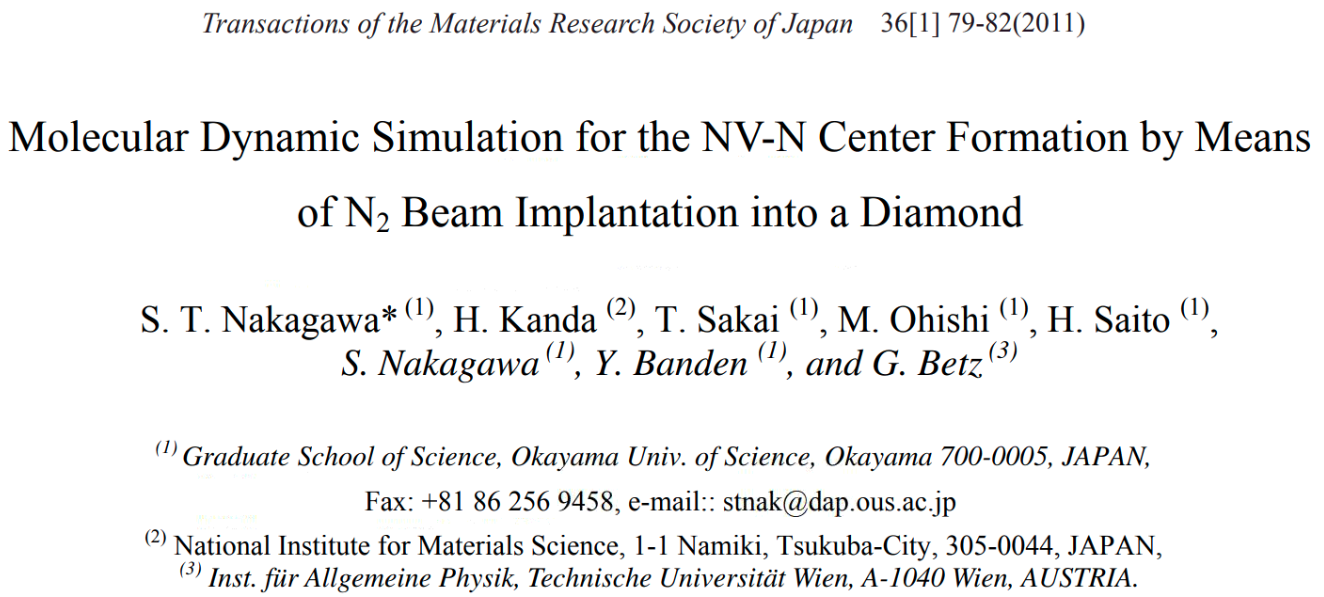
\includegraphics[width=0.7\textwidth]{pap0.png}
 \end{figure}
 \begin{itemize}
     \item NV Center $=$ change a carbon by nitrogen and remove another carbon in a neighbor.
     \item Change another carbon by nitrogen at relative distance $\textcolor{red}{\Rightarrow}$ NV-N Center (possible implementation of NOT gate).
     \item It was recomended to make a diamond lattice with the NV in center.
 \end{itemize}
 \end{frame}
 \begin{frame}{NV Centers MD Realisation.}
 \begin{itemize}
     \item NV-N can be built bombarding with N atoms this lattice via Montecarlo Method 
     \item Can be an easier form to put the second Nitrogen in \textcolor{green}{Lammps}?
     \item It would be needed the next libraries of \textcolor{green}{Lammps}:
     \begin{itemize}
         \item \textcolor{green}{spin}: Makes Magnetic Spin Simulations. Allows to modify the magnetic field.
         \item \textcolor{green}{gcmc}: Grand Canonical Monte Carlo simulation with interaction of an ideal gas (made of Nitrogen for our purposes).
     \end{itemize}
 \end{itemize}
\end{frame}
\begin{frame}{Abinitio NV Centers Theory}
\begin{figure}
 \centering
    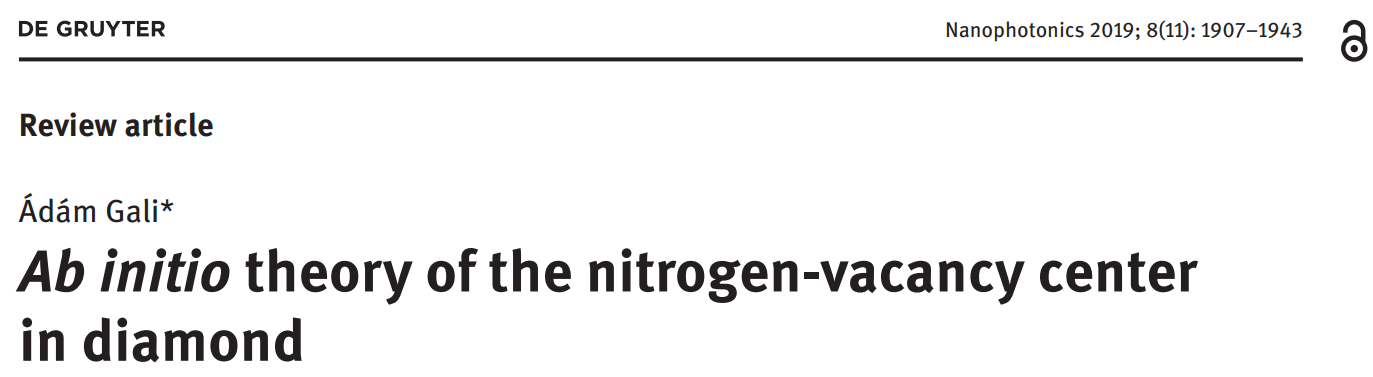
\includegraphics[width=0.7\textwidth]{pap1.png}
 \end{figure}
 \begin{itemize}
     \item The point defect of the NV Center is \textcolor{red}{Paramagnetic}
     \item The eigenstates of the NV center can be labeled by $C_{3v}$ symmetry irreducible representations (symmetry under rotation in $\frac{\pm 2\pi}{3}$ and  3 mirrors).
     \item It was required to see phonon interaction with the NV \textcolor{red}{$\Rightarrow$} \textcolor{green}{Phonolammps}
 \end{itemize}
\end{frame}
\begin{frame}{Abinitio NV Centers Theory}
 \begin{itemize}
     \item Abinitio simulation possible applications:
     \begin{itemize}
         \item Interaction with another lattices and point defects.
         \item Magnetooptical properties dependence of Thermodynamical changes (Temperature, Volume, Electromagnetic Field...)
     \end{itemize}
     \item The second application was very few explored \textcolor{red}{(!!!)}
     \item This papers gives Fermi Energies that can be used as a reference for future results.
 \end{itemize}
\end{frame}
\begin{frame}{Abinitio NV Centers Examples}
\begin{figure}
 \centering
    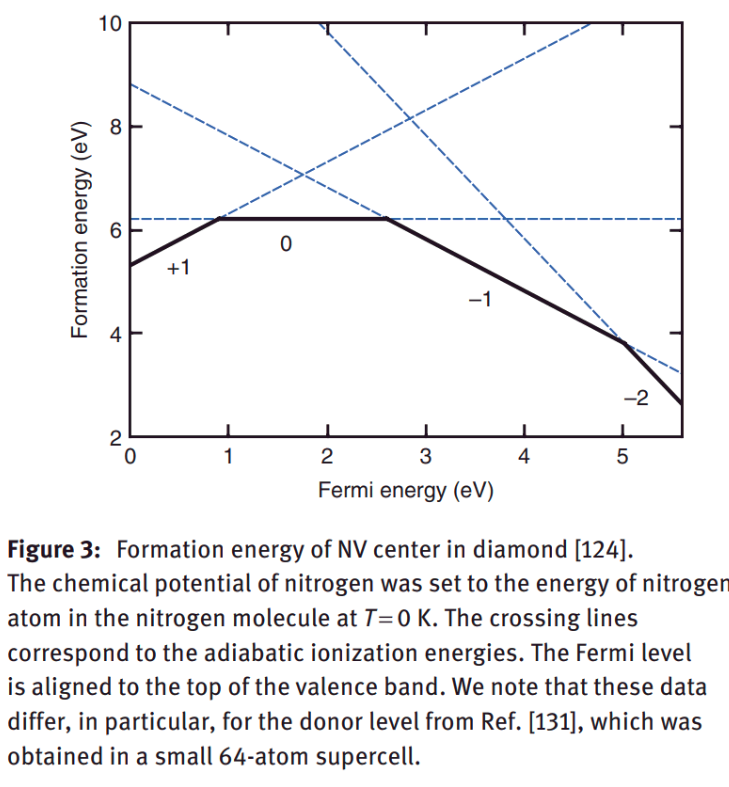
\includegraphics[width=0.7\textwidth]{Expected1.png}
 \end{figure}
\end{frame}
\title[NV-WR2]{NV Centers Weekly Report 2} 
\begin{frame}
\titlepage 
\end{frame}
\begin{frame}{First Principles Spin Calculation}
\begin{figure}
 \centering
    
\includegraphics[width=0.7\textwidth]{pap2.png}
 \end{figure}
  \begin{itemize}
     \item Electronically, point defect system can be modeled as two level systems with a defined optical frecuency transition.
     \item Definition: \textcolor{red}{ZPL: Zero Phonon Luminiscence} $=$ Difference between excited and ground state with zero phonons in the lattice. 
     \item Another possible check calculation: Hyperfine tensor (result of electron-nucleus coupling) \textcolor{red}{(!!!)}.
 \end{itemize}
\end{frame}
\begin{frame}{First Principles Bands Calculation}
\begin{figure}
 \centering
    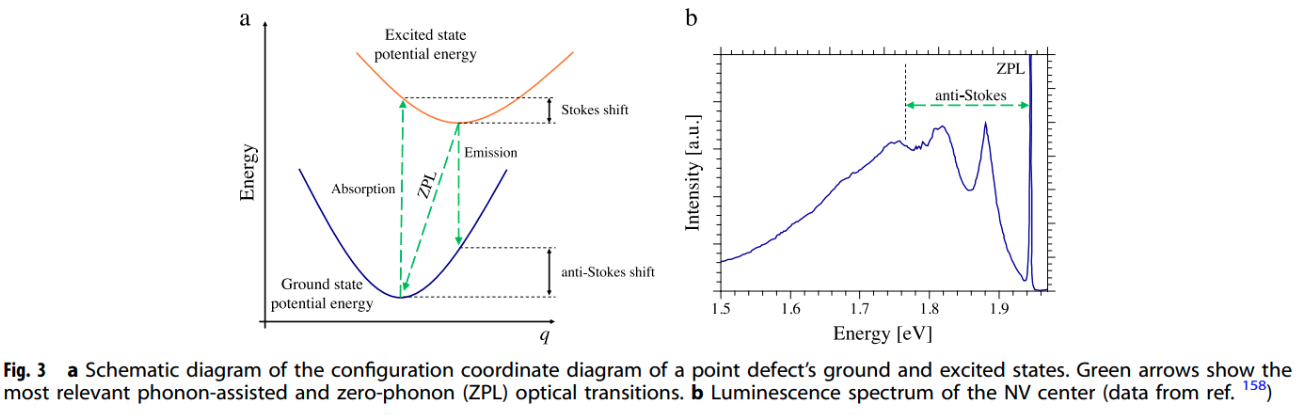
\includegraphics[width=0.9\textwidth]{zpl.png}
 \end{figure}
\begin{itemize}
    \item ZPL can be found in MD finding the energies for zero photons.
    \item Another relevant concept: \textcolor{red}{Luminiscence Spectrum}, seems to be a \textit{fingerprint} of the material.
\end{itemize} 
 \end{frame}

\begin{frame}{Initial Project}
\begin{enumerate}
    \item Measure vibrational modes of diamond crystal simulations using con \textcolor{green}{Phono\textcolor{green}{LAMMPS}} and comparing potentials \textcolor{green}{Tersoff}, \textcolor{green}{ReboScr}, \textcolor{green}{ReaxFF} y \textcolor{green}{COMB}.
    \item Add vacancies, measure modes again and compare with \textcolor{green}{DFT} results.
    \item Check for any potential if the results works (sequentially: \textcolor{green}{ReaxFF}, \textcolor{green}{COMB}, \textcolor{green}{Tersoff}). 
    \item Add nitrogen atoms to the system which gives the best results.
    \item Obtain (Spectral Function) $S_q$ and comparing it with experimental and \textcolor{green}{DFT} results.
    \item Make the same procedure for nanoclusters, materials with defects, dislocations...
     \end{enumerate}
\end{frame}

\begin{frame}{Thermodynamics and defect concentration}
\begin{figure}
 \centering
    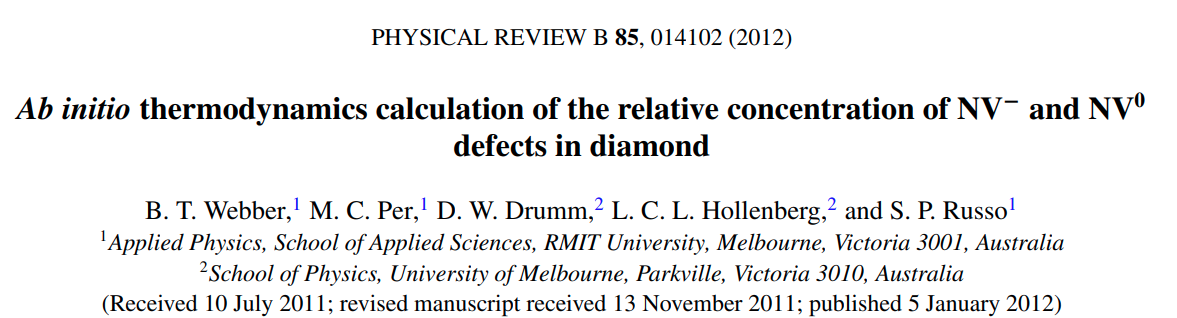
\includegraphics[width=0.7\textwidth]{pap4.png}
 \end{figure}
  \begin{itemize}
     \item It can be formed $NV^-$ and $NV^0$ defects in a diamond lattice
     \item For the applications (Decoherence, $QKD$, $QI$) it is needed to have a greater concentration of $NV^-$
     \item In Laboratory, NV Centers are made by \textit{thermal annealing}.
 \end{itemize}
\end{frame}
\begin{frame}{Thermodynamics and defect concentration}
\begin{itemize}
     \item \textcolor{red}{DFFE:} Defect Formation Free Energy \begin{equation}\Delta F_{f}^D=F^D-[F^H+\sum_d n_d\mu_d-\sum_h n_h\mu_h-q\mu_e]\end{equation}
     $n_h$: Host Atoms ,$n_d$: Defect Atoms, $\mu_d, \mu_e, \mu_h$: Chemical Pot.
     \item Relative DFEE:
     \begin{equation}\Delta F_f^{Rel}=\Delta F_f^{NV^-}-\Delta F_f^{NV^0}=F^{NV^-}-F^{NV^0}+q\mu_e\end{equation}
     \item  If $\Delta F_f^{Rel}>0$, the $NV^0$ centers are more stable thermodynamically. 
\end{itemize}
\end{frame}
\begin{frame}{Thermodynamics and defect concentration}
\begin{itemize}
     \item \textcolor{red}{Equilibrium Defect Concentration}: Directely related with DFFE \begin{equation}C^D (T)=n_ln_0e^{-\beta\Delta F_f^D}\end{equation}
     $n_l$: number of defects $n_0$: number of orientations by defect 
     \item A charge from a reservoir system (a pure diamond bulk) is needed to make a bulk with a defined concentration of $NV^-$
     \item \textcolor{red}{Relative Concentration}: Possible quantity to label simulations.
     \begin{equation}C^{rel}=\frac{C^{NV^-}}{C^{NV^0}}=\frac{(n_ln_0)^{NV^-}}{(n_ln_0)^{NV^0}}e^{-\beta\Delta F_f^{Rel}}\end{equation}
\end{itemize}
\end{frame}
\title[NV-WR3]{NV Centers Weekly Report 3} 
\begin{frame}
\titlepage 
\end{frame}
\begin{frame}{Vibrational and Electronic Dynamics}
\begin{figure}
 \centering
    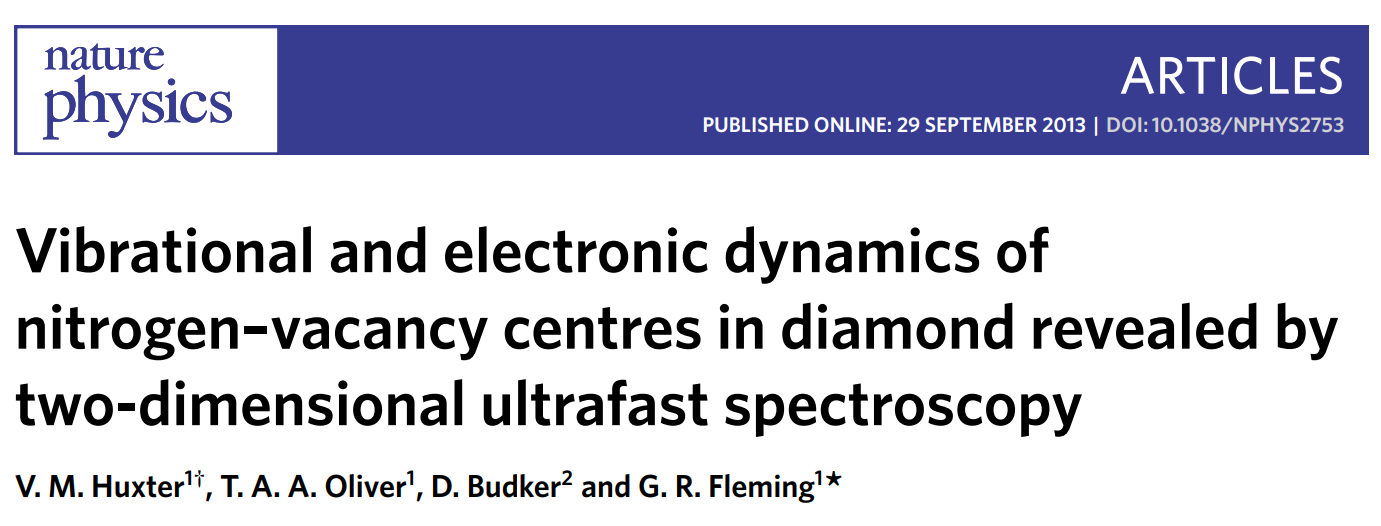
\includegraphics[width=0.7\textwidth]{pap6.png}
 \end{figure}
  \begin{itemize}
     \item It can be found using the next models:
     \begin{itemize}
         \item \textcolor{red}{GW Approximation (GWA}: Simplifying selfenergies.
         \item \textcolor{red}{Bethe-Salpeter Equation (BSE)}: Bound states of two particle system (aproximation of QFT).
         \item \textcolor{red}{Manybody Pertubation Theory (MBPT)}: Enough for optical excitation
     \end{itemize}
     \item The main goal: To find the \textcolor{red} {dynamics of the vibrational bath}, useful for understanding of optical dephasing and another optical induced effects.\textcolor{red}{(!!!)}
 \end{itemize}
\end{frame}
\begin{frame}{Vibrational and Electronic Dynamics}
\begin{itemize}
    \item Questions that this can solve:
    \begin{itemize}
        \item Is the vibrational and electronic dynamics of NV Centers an effectof such vibrational bath?
        \item Can the Dynamics of the vibrational bath to provoke ultrafast decay?
    \end{itemize}
    \item Experimentally, this dynamics can  be obtained by ultrafast measurements, called \textcolor{red}{2D Electronic Spectroscopy (2DES)}.
    \item In \textcolor{green}{DFT} simulations it was observed vibrational and electronic relaxations, reaching to a definition of \textcolor{red}{Absortion Spectra}
    \item The second derivative of Absortion Spectra is called \textcolor{red}{Vibronic Structure}. This structure is like a \textit{fingerprint} of the defect.
\end{itemize}
\end{frame}
\begin{frame}{NV Centers Transmision Luminescence}
\begin{figure}
 \centering
    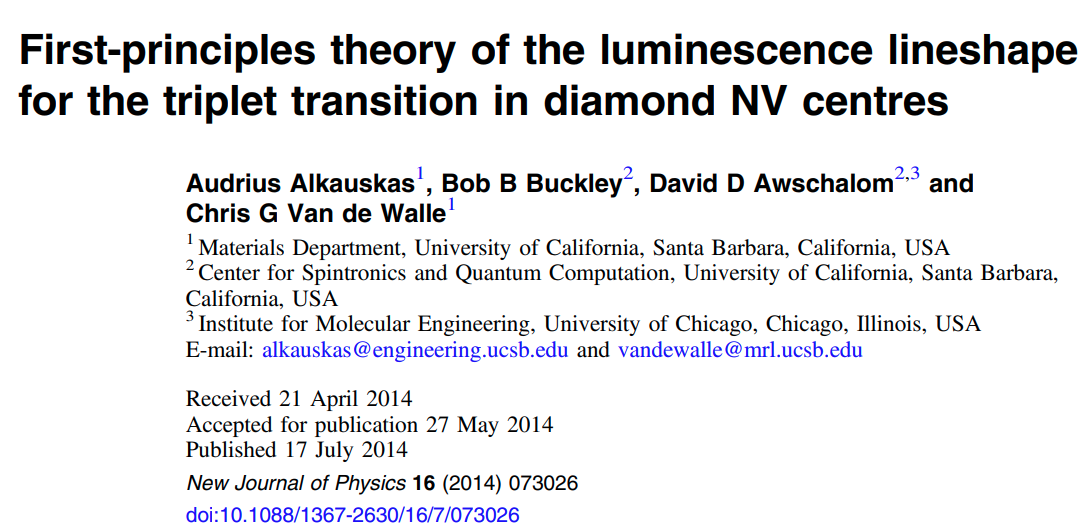
\includegraphics[width=0.9\textwidth]{pap8.png}
 \end{figure}
  \begin{itemize}
     \item Almost all the NV Centers applications are coming from the measurement of \textcolor{red}{photoluminiscence} between excited and ground states of de NV Center system as a function of another experimental variables.
 \end{itemize}
\end{frame}
\begin{frame}{NV Centers Transmision Luminescence}
  \begin{itemize}
    \item At low temperature the luminiscence band is a straight line in ZPL. 
    \item Alkausas obtained the luminiscence spectra for NV Centers using \textcolor{green}{DFT}. Can this spectra be obtained by \textcolor{green}{MD}? \textcolor{red}{(!!!)}
    \item The electron and the rest of the lattice form a \textcolor{red}{Jahn-Teller $E\otimes e$ system}, that can be defined roughly as a geometrical distortion of the bands of the system, reducing energy and symmetry.
 \end{itemize}
\end{frame}
\begin{frame}{NV Centers Transmision Luminescence}
  \begin{itemize}
    \item The Luminiscence Spectra analysis is made considering the following approximations:
    \begin{itemize}
        \item Normal modes that contributes to luminiscence are the bulk with defect ones, more that the beam ones.
        \item Modes in excited electronic state are the same than the ground electronic state.
    \end{itemize}
    \item The second approximation doesn't work at all for NV Centers. But it can be compared with experimental data to make corrections for the model.
    \item Luminiscence Spectra is related with \textcolor{red}{Spectral Density}. Finding one of them it can be derived the another:
    \begin{equation}S(\hslash\omega)=\sum_k S_k\delta(\hslash\omega-\hslash\omega_k)\end{equation}
 \end{itemize}
\end{frame}
\begin{frame}{Method for implementation of MD Simulation}
 Diamond samples realisation
  \begin{enumerate}
    \item Make diamond lattice samples in the potentials \textcolor{green}{Tersoff}, \textcolor{green}{Rebo}, \textcolor{green}{ReaxFF} y \textcolor{green}{COMB}.
    \item Take the library \textcolor{green}{gcmc} for bombarding a copy of the sample and obtaining NV and NV-N Systems
    \item Evaluate the stability of the all the samples in each potential (changes of phase, elastic variables).
 \end{enumerate}
\end{frame}
\begin{frame}{Method for implementation of MD Simulation}
  Lattice Measurements
  \begin{enumerate}
    \item Find the both \textit{fingerprints}: Luminiscence Spectrum and Vibrionic Structure using the \textcolor{green}{photon} and \textcolor{green}{PhonoLammps} libraries.
    \item Find the following properties: Hyperfine Tensor, Dynamics of Vibrational Bath.
    \item Evaluate the dependance of the properties of variables like Temperature, Pressure and External Magnetic Field
 \end{enumerate}
\end{frame}
\title[NV-WR4]{NV Centers Weekly Report 4} 
\begin{frame}
\titlepage 
\end{frame}
\begin{frame}{Lammps: Fix Phonon Command}
  \begin{itemize}
    \item The command \textcolor{green}{fix:phonon} depends of \textcolor{green}{PHONON} package (\textcolor{green}{Lammps} must be compiled with this package)
    \item This package allow to use a command that has a detailed command to take phonon dynamics. 
    \item This phonon dynamics can be taken to do band diagram user another code that it will explained later.
 \end{itemize}
\end{frame}
\begin{frame}{Lammps: Fix Phonon Command}
  \begin{itemize}
    \item Syntax of \textcolor{green}{fix phonon command}:
    \\ \textcolor{green}{fix 1 all phonon 10 5000 500000 GAMMA OUT nasr 100}
    \item Elements of syntax
    \begin{itemize}
        \item \textcolor{green}{10}: Timelapse between Green function measurements.
        \item \textcolor{green}{5000}: Lapse between measurements when dynamical matrix is obtained.
        \item \textcolor{green}{500000}: Lapse between measurements (Waiting time).
        \item \textcolor{green}{GAMMA}: Generate map info internally.
        \item \textcolor{green}{nasr 100}: Number of iterations to enforce acoustic sum rule.
    \end{itemize}
 \end{itemize}
\end{frame}
\begin{frame}{Lammps: Fix Phonon Command}
  \begin{itemize}
    \item Files used in every sample:
    \begin{itemize}
        \item \textcolor{green}{in.dia}: Generate a Diamond Bulk using any potential.
        \item \textcolor{green}{dia.out}: Output file made by \textcolor{green}{in.dia}
        \item \textcolor{green}{in.in}: Take \textcolor{green}{dia.out} and measure the phonon spectra for the lattice.
    \end{itemize}
    \item If it has obtained the phonon spectra, Can this spectra be visualized?
    \item It was needed a special tool for it.
 \end{itemize}
\end{frame}
\begin{frame}{Phana: Band Diagrams from Lammps Output}
  \begin{itemize}
    \item Phana is for \textit{Phonon Analyzer}, takes a dump file and converts it in a datafile ready for \textcolor{green}{Gnuplot}
    \item It is in \textcolor{green}{Lammps} folder, in \textcolor{green}{lammps/tools/USER/PHONON}
    \item It was needed \textcolor{green}{BLAS} and \textcolor{green}{LAPACK} library. This can be installed in \textcolor{green}{Linux} following \hyperlink{http://www.ifp.illinois.edu/grouper/clapack.html}{\textit{Illinois}}
    \item It was tested in my PC (2 cores) and repeated the installation in the COIC PC (12 cores).
 \end{itemize}
\end{frame}
\begin{frame}{Phana: Band Diagrams from Lammps Output}
  \begin{itemize}
    \item Phana is used putting the command 
    \\ \textcolor{green}{phana Out.bin.6000000 < in.disp}
    \item Elements of Syntax:
    \begin{itemize}
        \item \textcolor{green}{Out.bin.6000000}: Binary file result of \textcolor{green}{in.in}-
        \item \textcolor{green}{in.disp}: File with instructions for \textcolor{green}{Phana}
    \end{itemize}
    \item The \textcolor{green}{Phana} gives a file that, ran in \textcolor{green}{Gnuplot}, gives the band diagram.
 \end{itemize}
\end{frame}
\begin{frame}{Test: Theory of Bands for Diamond Bulk}
  \begin{itemize}
    \item For the \textcolor{green}{COMB}, \textcolor{green}{EDIP}, \textcolor{green}{aiREBO} and \textcolor{green}{Tersoff} potentials:
    \begin{enumerate}
        \item Modify script from aC module to give diamond structure thermodynamically stable.
        \item Run it as \textcolor{green}{in.dia} files, giving the \textcolor{green}{dia.out} required
        \item Follow the method shown in the last slides.
    \end{enumerate}
    \item The band diagram for diamond can be found on references, for comparison with simulation data
    \item If it has found error, analise and fix it.
 \end{itemize}
\end{frame}

\title[NV-WR5]{NV Centers Weekly Report 5} 
\begin{frame}
\titlepage 
\end{frame}
\begin{frame}{Development of To-Do list}
\begin{itemize}
\item bla
\begin{itemize}
\item[\done] blub
\item[\fail] bla
\item[\pend] blo
\end{itemize}
\item blub
\end{itemize}
\end{frame} 

\title[NV-WR6]{NV Centers Weekly Report 6} 
\begin{frame}
\titlepage 
\end{frame}
\begin{frame}{Development of To-Do list}
\begin{itemize}
\item bla
\begin{itemize}
\item[\done] blub
\item[\fail] bla
\item[\pend] blo
\end{itemize}
\item blub
\end{itemize}
\end{frame} 

\title[NV-WR7]{NV Centers Weekly Report 7} 
\begin{frame}
\titlepage 
\end{frame}
\begin{frame}{Development of To-Do list}
\begin{itemize}
\item bla
\begin{itemize}
\item[\done] blub
\item[\fail] bla
\item[\pend] blo
\end{itemize}
\item blub
\end{itemize}
\end{frame} 

\title[NV-WR8]{NV Centers Weekly Report 8} 
\begin{frame}
\titlepage 
\end{frame}
\begin{frame}{Development of To-Do list}
\begin{itemize}
\item bla
\begin{itemize}
\item[\done] blub
\item[\fail] bla
\item[\pend] blo
\end{itemize}
\item blub
\end{itemize}
\end{frame} 

\end{document}
